\begin{figure}[t!]
    \centering

    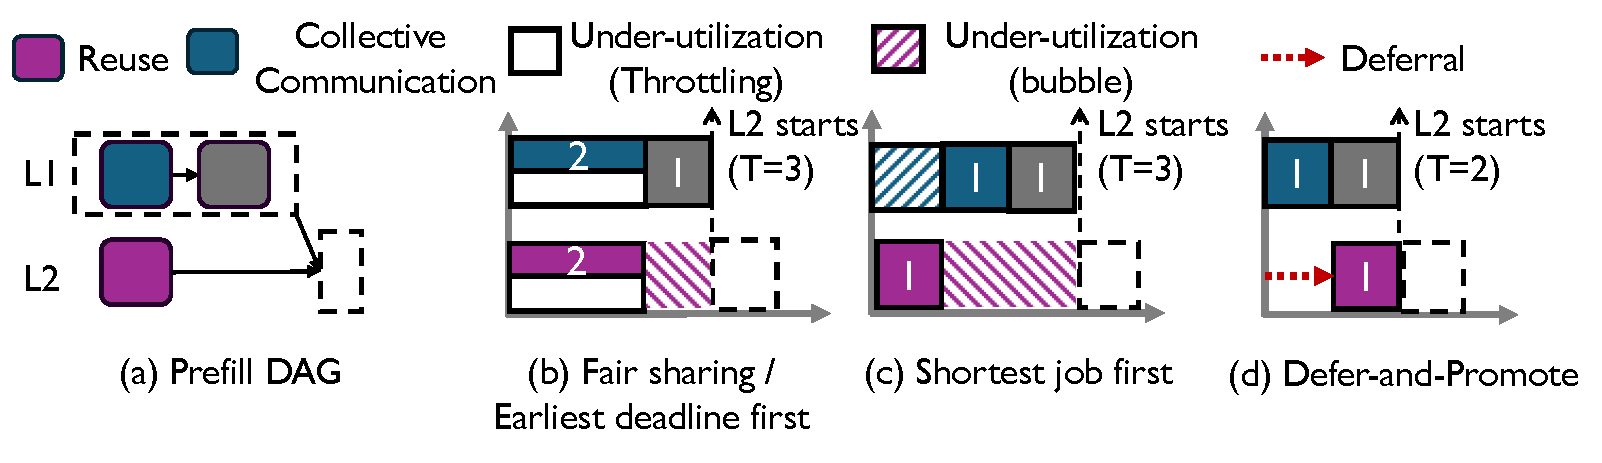
\includegraphics[width=\linewidth]{figures/methodology/IntraContentionExample-A.pdf}
    \caption{\textbf{请求内争用（入口）场景下不同调度策略的对比。}
    (a) 第 1 层执行期间的入口端口争用。
    (b)-(c) FS/SJF/EDF 将第 2 层启动时间延迟到 $T=3$。
    (d) \textit{延后并提升}策略将第 2 层启动时间提前到 $T=2$（缩短 33\%）。}
    \label{fig:meth:intraA}

    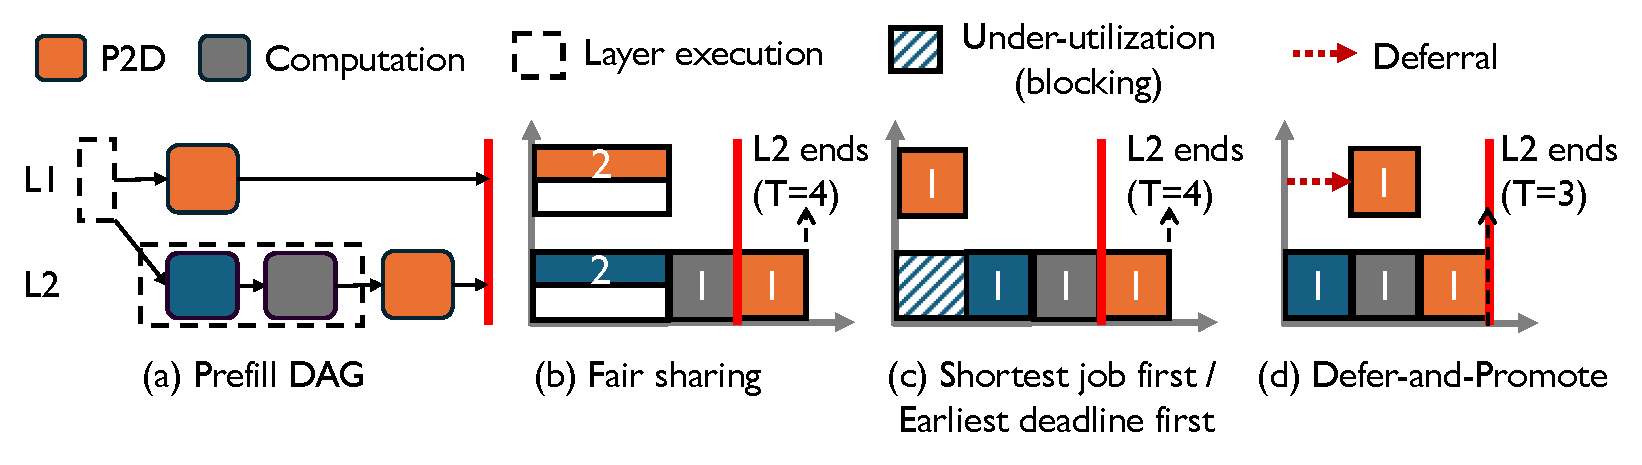
\includegraphics[width=\linewidth]{figures/methodology/IntraContentionExample-B.pdf}
    \caption{\textbf{请求内争用（出口）场景下不同调度策略的对比。}
    (a) 第 2 层执行期间的出口端口争用。
    (b)-(c) FS/SJF/EDF 将第 2 层完成时间延迟到 $T=4$。
    (d) \textit{延后并提升}策略将第 2 层结束时间缩短到 $T=3$（降低 25\%）。}
    \label{fig:meth:intraB}
\end{figure}
